\documentclass{article}

\usepackage[%
    left=0.5in,%
    right=0.5in,%
    top=0.5in,%
    bottom=0.5in,%
]{geometry}%
\usepackage{minitoc}
\usepackage{multicol}
\usepackage{graphicx}
\usepackage{fixltx2e}
\usepackage{listings}
\usepackage{color}
\usepackage{hyperref}
    \hypersetup{ colorlinks = true, linkcolor = blue }
\usepackage{blindtext}
\definecolor{lightgray}{gray}{0.9}
\graphicspath{ {./} }
\usepackage{listings}
\usepackage{color}

\definecolor{dkgreen}{rgb}{0,0.6,0}
\definecolor{gray}{rgb}{0.5,0.5,0.5}
\definecolor{mauve}{rgb}{0.58,0,0.82}

\lstset{frame=tb,
  language=Java,
  aboveskip=3mm,
  belowskip=3mm,
  showstringspaces=false,
  columns=flexible,
  basicstyle={\small\ttfamily},
  numbers=none,
  numberstyle=\tiny\color{gray},
  keywordstyle=\color{blue},
  commentstyle=\color{dkgreen},
  stringstyle=\color{mauve},
  breaklines=true,
  breakatwhitespace=true,
  tabsize=3
}

\newcommand{\inlinecode}[2]{\colorbox{lightgray}{\lstinline
[language=#1]$#2$}}
\newcommand{\worddef}[1]{\hyperref[sec:reference]{\textit{#1}}}

\begin{document}

\section{FW All-Pairs SPs}

\subsection{Data structure}
\texttt{d(i,j,k) =}
\begin{itemize}
	\item shortest distance between nodes i and j
	\item using only the nodes {1,…,k} as potential allowed intermediary points
\end{itemize}

\subsection{Initialisation of data structure}
\begin{flushleft}
\texttt{d(i,j,0) =} best distance between nodes i and j, but not using any intermediate nodes, so only using a single edge, hence \texttt{d(i,j,0) = w(i,j)} if there is an edge i to j, otherwise \texttt{Inf}
\end{flushleft}

\subsection{All-Pairs SPs}
\begin{itemize}
	\item Now suppose that we add the node ‘n1’ to the set of nodes that can be intermediates, i.e. consider k = 1
	\item Best path is now the best of “either direct, or via n1.”
	\item \texttt{d(i,j,1)} \\
		= \texttt{min ( d(i,j,0), w(i,n1) + w(n1,j) )} \\
		= \texttt{min ( d(i,j,0), d(i,n1,0) + d(n1,j,0) )} \\
\end{itemize}
\begin{center}
	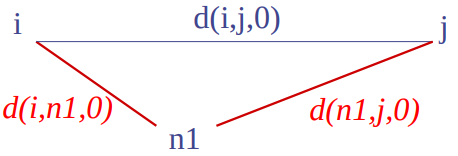
\includegraphics[scale=0.5]{pair_shortest.png}
\end{center}

\begin{itemize}
	\item Now suppose that we add the new node “(k+1)” to the set of “via nodes” that can be intermediates, but have already considered k of them
	\item Best path is now either direct using only the k ‘via nodes’ already accounted for, or else also via node ‘k+1’ (and using the previous k via’s)
	\item \texttt{d(i,j,k+1) = min ( d(i,j,k), d(i,k+1,k) + d(k+1,j,k) )}
\end{itemize}
\begin{center}
	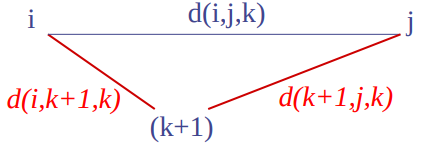
\includegraphics[scale=0.5]{k+1_shortest.png}
\end{center}

\subsection{Equations}
\begin{itemize}
	\item \texttt{d(i,j,0)} \\
		= \texttt{w(i,j)} if there is an edge i to j \\
		= \texttt{Inf} otherwise
	\item \texttt{d(i,j,k+1) = min ( d(i,j,k), d(i,k+1,k) + d(k+1,j,k) )}
	\item \texttt{d( i, i ) = 0 forall i}
\end{itemize}

\subsection{Complexity}
\begin{flushleft}
Because we have 3 variables, i,j,k we will need 3 levels nested for loop, where \texttt{i = j = k = |V|}, so worst case is $O(|V|^3)$
\end{flushleft}

\subsection{Digraphs (Directional graphs)}
\begin{flushleft}
The algorithm also works on directional graphs.The initial matrix \texttt{d(i,j,0)} need not be symmetric, but then
the remaining calculations use exactly the same formulas
\end{flushleft}

\subsection{Negative edges}
\begin{flushleft}
FW even works if some (directed) edge weights are negative
\begin{itemize}
	\item BUT it is essential that there are \textbf{no cycles of total negative weight}
	\item Otherwise simply repeatedly following around the negative cycle may reduce lengths to be as negative as desired, so there is \textbf{no shortest path}
\end{itemize}
\end{flushleft}

\end{document}
